\documentclass{article}
\usepackage[utf8]{inputenc}
\usepackage[vietnamese,english]{babel}
\usepackage{times}
\usepackage{amsmath,amssymb}
\usepackage{tabularx}
\usepackage{array}
\usepackage{booktabs}
\usepackage{graphicx}
\usepackage{xcolor}
\usepackage{tikz}
\usepackage[version=4]{mhchem}
\usepackage[
  paperwidth=29.7cm,
  paperheight=16.706cm,
  top=0.9cm,
  bottom=0.9cm,
  left=1.2cm,
  right=1.2cm,
  footskip=0pt,
  headheight=0pt,
  headsep=0pt
]{geometry}

\pagestyle{empty}
\setlength{\parindent}{0pt}
\setlength{\parskip}{0pt}

% Định nghĩa màu sắc thương hiệu Thầy Thạnh
\definecolor{brandGreen}{RGB}{46, 125, 50}
\definecolor{brandRed}{RGB}{211, 47, 47}
\definecolor{brandBlue}{RGB}{21, 101, 192}

\begin{document}
\selectlanguage{vietnamese}

% ==============================================================================
% SLIDE 1: TRANG TIÊU ĐỀ
% ==============================================================================
\begin{center}
\vspace*{0.5cm}
{\fontsize{24}{30}\selectfont \textbf{TRUNG TÂM LUYỆN THI HÓA HỌC THẦY THẠNH}}\\[0.6cm]
{\fontsize{34}{42}\selectfont \textbf{\color{brandGreen}ĐỀ KIỂM TRA ĐỊNH KÌ HÓA HỌC 12 -- ĐỀ GỐC LẦN 11}}\\[0.4cm]
{\fontsize{26}{34}\selectfont \textbf{BỘ CÂU HỎI THEO MA TRẬN ĐỀ THI TỐT NGHIỆP THPT QUỐC GIA}}\\[0.6cm]
{\fontsize{21}{27}\selectfont \textit{Cho biết nguyên tử khối: H = 1; C = 12; N = 14; O = 16; Na = 23; Mg = 24; Al = 27; P = 31;}}\\[0.15cm]
{\fontsize{21}{27}\selectfont \textit{S = 32; Cl = 35,5; K = 39; Ca = 40; Fe = 56; Cu = 64; Zn = 65; Br = 80; Ag = 108; Ba = 137.}}\\[0.8cm]
{\fontsize{24}{30}\selectfont \textbf{\color{brandRed}Thầy TRẦN VĂN THẠNH -- 0777.470.803}}\\[0.3cm]
{\fontsize{20}{26}\selectfont CS1: 6/15 Nguyễn Hoàng, P. Kim Long, TP Huế \quad | \quad CS2: 24 Đặng Thái Thân, TP Huế}
\end{center}
\newpage

% ==============================================================================
% PHẦN I. CÂU TRẮC NGHIỆM NHIỀU PHƯƠNG ÁN LỰA CHỌN
% ==============================================================================

% SLIDE 2: CÂU 1 (Bài toán tráng bạc ruột phích Rạng Đông)
\fontsize{27}{36}\selectfont
\textbf{Câu 1.} Nhà máy Rạng Đông là nhà máy sản xuất phích nước hàng đầu của nước ta với nhiều mặt hàng quan trọng. Sản lượng năm 2003 đạt được là 7 triệu ruột phích. Để tráng được số lượng ruột phích như trên với mỗi ruột phích có diện tích bề mặt là $0{,}35\text{ m}^2$, độ dày lớp bạc là $0{,}1\ \mu\text{m}$ thì năm 2003 nhà máy cần dùng $m$ tấn glucose tác dụng với lượng dư dung dịch $\ce{AgNO3}$ trong $\ce{NH3}$. Biết hiệu suất phản ứng tráng bạc là $70\%$ và khối lượng riêng của bạc là $10{,}49\text{ g/cm}^3$. Giá trị của $m$ là bao nhiêu? (kết quả làm tròn đến hàng phần trăm)
\vspace{16pt}

\begin{tabularx}{\linewidth}{@{}X X X X@{}}
\textbf{A.} 6,12. & \textbf{B.} 3,6. & \textbf{C.} 3,06. & \textbf{D.} 6,21.
\end{tabularx}
\vspace*{\fill}
\newpage

% SLIDE 3: CÂU 2 & CÂU 3 (Đã tinh chỉnh để vừa khít 1 slide)
\fontsize{25}{32}\selectfont
\textbf{Câu 2.} Phát biểu nào sau đây là đúng?
\vspace{4pt}

\begin{tabularx}{\linewidth}{@{}X X@{}}
\textbf{A.} Ala-Gly hoà tan $\ce{Cu(OH)2}$ cho màu tím. & \textbf{B.} Glutamic acid có tính lưỡng tính.\\[4pt]
\textbf{C.} Peptide Ala-Gly-Ala có ba liên kết peptide. & \textbf{D.} Hemoglobin là protein hình sợi.
\end{tabularx}

\vspace*{\fill}

\textbf{Câu 3.} Cho hình vẽ sau của amino acid X trong môi trường $\text{pH} = 6$ dưới tác dụng của điện trường:
\vspace{4pt}

\begin{center}
\begin{tikzpicture}[scale=0.8]
  \fill[yellow!35] (0,0) rectangle (9,1.3);
  \draw[blue!70!black, line width=1.5pt] (0,0) rectangle (9,1.3);
  \draw[green!60!black, fill=green!40, line width=1.2pt] (-0.6,0.65) circle (0.38);
  \node at (-0.6,0.65) {\large \bfseries $-$};
  \draw[green!60!black, fill=green!40, line width=1.2pt] (9.6,0.65) circle (0.38);
  \node at (9.6,0.65) {\large \bfseries $+$};
  \fill[red] (0.8,0.65) circle (0.32);
\end{tikzpicture}
\end{center}
\vspace{2pt}
X có thể là
\vspace{4pt}

\begin{tabularx}{\linewidth}{@{}X X X X@{}}
\textbf{A.} Glutamic acid. & \textbf{B.} Glycine. & \textbf{C.} Alanine. & \textbf{D.} Lysine.
\end{tabularx}
\vspace*{\fill}
\newpage

% SLIDE 4: CÂU 4 & CÂU 5
\fontsize{28}{38}\selectfont
\textbf{Câu 4.} Hợp chất $\ce{CH3CH2NH2}$ có tên thay thế là
\vspace{6pt}

\begin{tabularx}{\linewidth}{@{}X X@{}}
\textbf{A.} ethylamine. & \textbf{B.} $N$-methylmethanamine.\\[6pt]
\textbf{C.} methylamine. & \textbf{D.} ethanamine.
\end{tabularx}

\vspace*{\fill}

\textbf{Câu 5.} Aniline tác dụng với $(\ce{HNO2} + \ce{HCl})$ ở $0 - 5^\circ\text{C}$ theo phương trình sau đây:
\vspace{4pt}
\begin{center}
$\ce{C6H5NH2 + HONO + HCl ->[0 - 5^\circ\text{C}] X + 2H2O}$
\end{center}
\vspace{4pt}
Chất X có công thức cấu tạo là
\vspace{6pt}

\begin{tabularx}{\linewidth}{@{}X X@{}}
\textbf{A.} $[\ce{C6H5NH3}]^+\ce{Cl}^-$. & \textbf{B.} $[\ce{C6H5NH2}]^+\ce{Cl}^-$.\\[6pt]
\textbf{C.} $[\ce{C6H5N2H}]^+\ce{Cl}^-$. & \textbf{D.} $[\ce{C6H5N2}]^+\ce{Cl}^-$.
\end{tabularx}
\vspace*{\fill}
\newpage

% SLIDE 5: CÂU 6 & CÂU 7
\fontsize{27}{36}\selectfont
\textbf{Câu 6.} Glucose có thể lên men tạo lactic acid có trong sữa chua qua phản ứng nào sau đây?
\vspace{6pt}

\begin{tabularx}{\linewidth}{@{}X@{}}
\textbf{A.} $\ce{C6H12O6 ->[\text{enzyme}] 2C2H5OH + 2CO2}$.\\[5pt]
\textbf{B.} $\ce{C6H12O6 ->[\text{enzyme}] 2CH3-CHOH-COOH}$.\\[5pt]
\textbf{C.} $\ce{HOCH2[CHOH]4CHO + Br2 + H2O -> HOCH2[CHOH]4COOH + 2HBr}$.\\[5pt]
\textbf{D.} $\ce{2C6H12O6 + Cu(OH)2 -> (C6H11O6)2Cu + 2H2O}$.
\end{tabularx}

\vspace*{\fill}

\textbf{Câu 7.} Số nguyên tử nitrogen có trong phân tử peptide Lys-Gly-Ala?
\vspace{8pt}

\begin{tabularx}{\linewidth}{@{}X X X X@{}}
\textbf{A.} 4. & \textbf{B.} 3. & \textbf{C.} 2. & \textbf{D.} 5.
\end{tabularx}
\vspace*{\fill}
\newpage

% SLIDE 6: CÂU 8 & CÂU 9
\fontsize{28}{37}\selectfont
\textbf{Câu 8.} Đun nóng $0{,}1\text{ mol}$ một ester đơn chức X với $135\text{ mL}$ dung dịch $\ce{NaOH}\ 1\text{M}$ đến khi phản ứng xảy ra hoàn toàn, cô cạn dung dịch thu được ethyl alcohol và $8{,}2\text{ gam}$ chất rắn khan. Công thức cấu tạo của X là
\vspace{8pt}

\begin{tabularx}{\linewidth}{@{}X X X X@{}}
\textbf{A.} $\ce{HCOOC2H5}$. & \textbf{B.} $\ce{HCOOCH3}$. & \textbf{C.} $\ce{C2H3COOC2H5}$. & \textbf{D.} $\ce{CH3COOC2H5}$.
\end{tabularx}

\vspace*{\fill}

\textbf{Câu 9.} Chất X được tổng hợp bởi thực vật và chiếm khoảng $90\%$ khối lượng sợi bông. X là
\vspace{8pt}

\begin{tabularx}{\linewidth}{@{}X X X X@{}}
\textbf{A.} Saccharose. & \textbf{B.} Cellulose. & \textbf{C.} Tinh bột. & \textbf{D.} Maltose.
\end{tabularx}
\vspace*{\fill}
\newpage

% SLIDE 7: CÂU 10 & CÂU 11
\fontsize{29}{39}\selectfont
\textbf{Câu 10.} Nhỏ vài giọt dung dịch iodine vào lát cắt củ khoai tây, ta thấy tại lát cắt củ khoai tây chuyển màu
\vspace{8pt}

\begin{tabularx}{\linewidth}{@{}X X X X@{}}
\textbf{A.} đỏ. & \textbf{B.} da cam. & \textbf{C.} xanh tím. & \textbf{D.} nâu đen.
\end{tabularx}

\vspace*{\fill}

\textbf{Câu 11.} Isopropyl formate là một ester có trong cà phê Arabica (còn gọi là cà phê chè). Công thức của isopropyl formate là
\vspace{8pt}

\begin{tabularx}{\linewidth}{@{}X X@{}}
\textbf{A.} $\ce{HCOOCH(CH3)2}$. & \textbf{B.} $\ce{HCOOCH2CH2CH3}$.\\[8pt]
\textbf{C.} $\ce{HCOOCH3}$. & \textbf{D.} $\ce{HCOOCH2CH3}$.
\end{tabularx}
\vspace*{\fill}
\newpage

% SLIDE 8: CÂU 12 & CÂU 13
\fontsize{28}{37}\selectfont
\textbf{Câu 12.} Cho các ester sau: ethyl formate (1); vinyl acetate (2); triolein (3); methyl acrylate (4); phenyl acetate (5). Dãy gồm các ester đều phản ứng được với dung dịch $\ce{NaOH}$ dư, đun nóng sinh ra alcohol là
\vspace{8pt}

\begin{tabularx}{\linewidth}{@{}X X X X@{}}
\textbf{A.} (2), (3), (5). & \textbf{B.} (3), (4), (5). & \textbf{C.} (1), (2), (3). & \textbf{D.} (1), (3), (4).
\end{tabularx}

\vspace*{\fill}

\textbf{Câu 13.} Chất nào sau đây vừa tác dụng với dung dịch $\ce{NaOH}$, vừa tác dụng với dung dịch $\ce{HCl}$?
\vspace{8pt}

\begin{tabularx}{\linewidth}{@{}X X@{}}
\textbf{A.} Aniline. & \textbf{B.} Phenylammonium chloride.\\[8pt]
\textbf{C.} Glutamic acid. & \textbf{D.} Sodium acetate.
\end{tabularx}
\vspace*{\fill}
\newpage

% SLIDE 9: CÂU 14 (Công thức beta-glucose)
\fontsize{28}{36}\selectfont
\textbf{Câu 14.} Công thức nào dưới đây phù hợp với công thức cấu tạo của $\beta$-glucose?
\vspace{10pt}

\begin{center}
\begin{tabular}{cccc}
\textbf{A.} & \textbf{B.} & \textbf{C.} & \textbf{D.} \\[4pt]
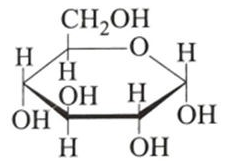
\includegraphics[height=4.3cm]{images_de_goc_11/cau14_opt_A.png} \hspace{0.3cm} &
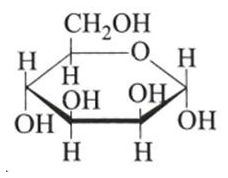
\includegraphics[height=4.3cm]{images_de_goc_11/cau14_opt_B.png} \hspace{0.3cm} &
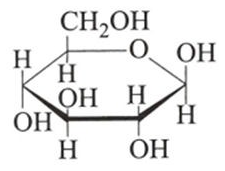
\includegraphics[height=4.3cm]{images_de_goc_11/cau14_opt_C.png} \hspace{0.3cm} &
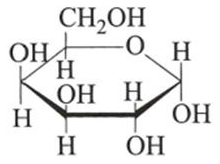
\includegraphics[height=4.3cm]{images_de_goc_11/cau14_opt_D.png}
\end{tabular}
\end{center}
\vspace*{\fill}
\newpage

% SLIDE 10: CÂU 15 (Đường huyết - tinh chỉnh vừa khít 1 slide)
\fontsize{24}{31}\selectfont
\textbf{Câu 15.} Trong máu người trưởng thành, khỏe mạnh vào lúc đói (8 giờ sau ăn) có lượng đường huyết trong khoảng $4{,}4 - 7{,}2\text{ mmol/L}$ (theo quyết định số 5481/QĐ-BYT ngày 30/12/2020 của Bộ Y tế). Cho các nhận định sau:
\vspace{5pt}

\begin{tabularx}{\linewidth}{@{}X@{}}
(a) Lượng đường huyết là lượng đường glucose trong máu.\\[3pt]
(b) Kết quả xét nghiệm đường huyết của anh A vào buổi sáng (lúc chưa ăn) là $152\text{ mg/dL}$ (biết $1\text{ L} = 10\text{ dL}$). Anh A có lượng đường huyết thấp hơn mức giới hạn bình thường.\\[3pt]
(c) Lúc đói nếu ăn thực phẩm chứa tinh bột thì lượng đường huyết sẽ tăng trong một khoảng thời gian nhất định.\\[3pt]
(d) Khi bị hạ đường huyết thì nên uống một cốc nước đường ấm.
\end{tabularx}
\vspace{4pt}
Số nhận định đúng là
\vspace{6pt}

\begin{tabularx}{\linewidth}{@{}X X X X@{}}
\textbf{A.} 2. & \textbf{B.} 1. & \textbf{C.} 3. & \textbf{D.} 4.
\end{tabularx}
\vspace*{\fill}
\newpage

% SLIDE 11: CÂU 16 & CÂU 17
\fontsize{29}{38}\selectfont
\textbf{Câu 16.} Công thức của chất béo trong các chất sau là?
\vspace{6pt}

\begin{tabularx}{\linewidth}{@{}X X@{}}
\textbf{A.} $(\ce{C17H35COO})_3\ce{C3H5}$. & \textbf{B.} $\ce{CH3COOCH2C6H5}$.\\[6pt]
\textbf{C.} $\ce{C15H31COOCH3}$. & \textbf{D.} $(\ce{C17H33COO})_2\ce{C2H4}$.
\end{tabularx}

\vspace*{\fill}

\textbf{Câu 17.} Chất béo là thức ăn quan trọng của con người, là nguồn cung cấp dinh dưỡng và năng lượng đáng kể cho cơ thể. Ngoài ra, một lượng lớn chất béo được dùng trong công nghiệp để sản xuất
\vspace{6pt}

\begin{tabularx}{\linewidth}{@{}X X@{}}
\textbf{A.} glucose và glycerol. & \textbf{B.} glucose và ethanol.\\[6pt]
\textbf{C.} xà phòng và glycerol. & \textbf{D.} xà phòng và ethanol.
\end{tabularx}
\vspace*{\fill}
\newpage

% SLIDE 12: CÂU 18
\fontsize{29}{39}\selectfont
\textbf{Câu 18.} Khi sử dụng xà phòng có thành phần chính là sodium stearate trong nước cứng, hiệu quả giặt rửa bị giảm đáng kể do tạo thành các kết tủa. Một trong những chất kết tủa đó là
\vspace{16pt}

\begin{tabularx}{\linewidth}{@{}X X@{}}
\textbf{A.} $\ce{C17H35COONa}$. & \textbf{B.} $(\ce{CH3COO})_2\ce{Mg}$.\\[16pt]
\textbf{C.} $(\ce{C17H35COO})_2\ce{Ca}$. & \textbf{D.} $\ce{C15H31COONa}$.
\end{tabularx}
\vspace*{\fill}
\newpage

% ==============================================================================
% PHẦN II. CÂU TRẮC NGHIỆM ĐÚNG / SAI (1 CÂU / SLIDE)
% ==============================================================================

% SLIDE 13: CÂU 1 (Điều chế ethyl acetate - tinh chỉnh vừa khít 1 slide)
\fontsize{23}{30}\selectfont
\textbf{Câu 1.} Một nhóm học sinh đã thực hiện phản ứng điều chế ethyl acetate từ nguyên liệu ban đầu là acetic acid và ethanol trong phòng thí nghiệm. Khi phản ứng kết thúc, nhóm đã thu được hỗn hợp sản phẩm gồm ethyl acetate, acetic acid và ethanol còn dư theo phương trình hoá học:
\begin{center}
$\ce{CH3COOH + C2H5OH <=>[H2SO4 \text{ đặc},\ t^\circ] CH3COOC2H5 + H2O}$
\end{center}
\vspace{4pt}

\begin{tabularx}{\linewidth}{@{}X r@{}}
a) Có thể thay dung dịch sulfuric acid đặc bằng dung dịch hydrochloric acid đặc. & $[\quad]$\\[4pt]
b) Thực hiện phản ứng ester hóa giữa $4{,}6\text{ gam}$ ethyl alcohol với lượng dư acetic acid, thu được $4{,}4\text{ gam}$ ester. Hiệu suất phản ứng ester hóa là $50\%$. & $[\quad]$\\[4pt]
c) Do diethyl ether có nhiệt độ sôi thấp hơn nhiều so với ethyl acetate ($34{,}6^\circ\text{C}$ so với $77{,}1^\circ\text{C}$) nên để thu được ethyl acetate có thể dùng nước nóng liên tục tưới lên bình cầu trong phương pháp chưng cất đơn giản để tách ethyl acetate ra khỏi dung môi diethyl ether sau khi chiết. & $[\quad]$\\[4pt]
d) Phản ứng trên được gọi là phản ứng xà phòng hóa. & $[\quad]$
\end{tabularx}
\vspace*{\fill}
\newpage

% SLIDE 14: CÂU 2 (Methionine)
\fontsize{24}{31}\selectfont
\textbf{Câu 2.} Methionine là một amino acid thiết yếu, được tìm thấy trong nhiều protein của thức ăn, mô và cơ quan của cơ thể con người. Methionine có công thức cấu tạo như hình bên:
\vspace{3pt}

\begin{center}
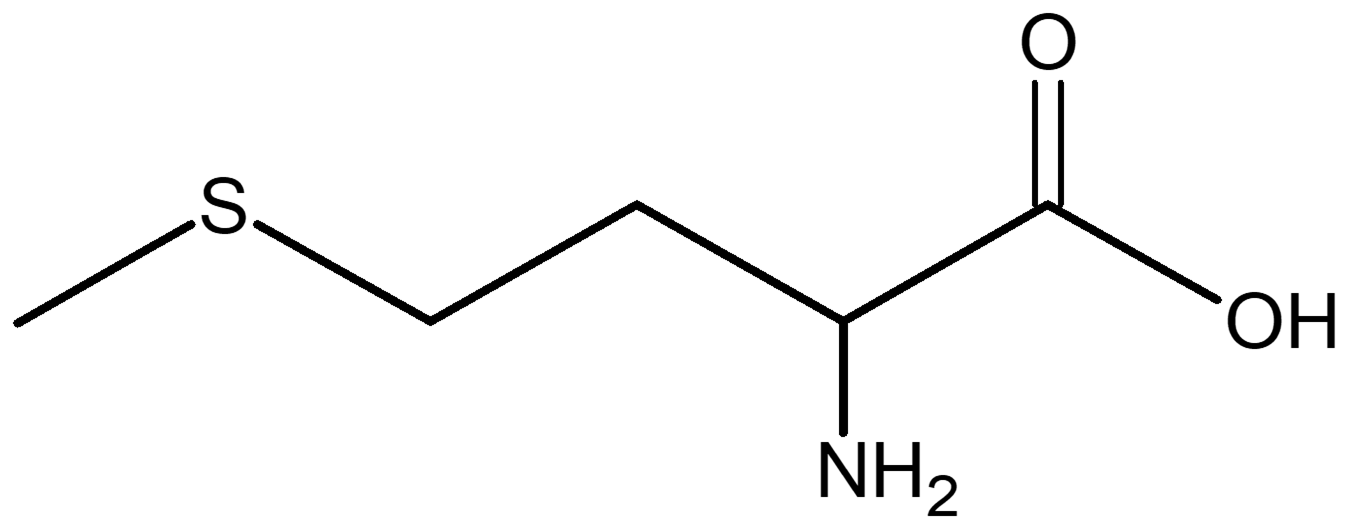
\includegraphics[height=2.6cm]{images_de_goc_11/methionine_clean.png}
\end{center}
\vspace{2pt}
Biết nhóm $\ce{CH3-S\bond{-}}$ có tên là methylthio.
\vspace{4pt}

\begin{tabularx}{\linewidth}{@{}X r@{}}
a) Phân tử methionine có 12 nguyên tử hydrogen. & $[\quad]$\\[5pt]
b) Methionine là $\alpha$-amino acid. & $[\quad]$\\[5pt]
c) Thức ăn giàu methionine có thể tìm thấy ở trứng, cá, thịt,... & $[\quad]$\\[5pt]
d) Methionine có tên thay thế là 2-amino-4-(methylthio)butanoic acid. & $[\quad]$
\end{tabularx}
\vspace*{\fill}
\newpage

% SLIDE 15: CÂU 3 (Thí nghiệm thủy phân cellulose - tinh chỉnh vừa khít 1 slide)
\fontsize{22}{28}\selectfont
\textbf{Câu 3.} Tiến hành thí nghiệm thủy phân cellulose (bông) bằng dung dịch acid ($\ce{H2SO4}\ 70\%$) như hình mô tả:
\vspace{2pt}

\begin{center}
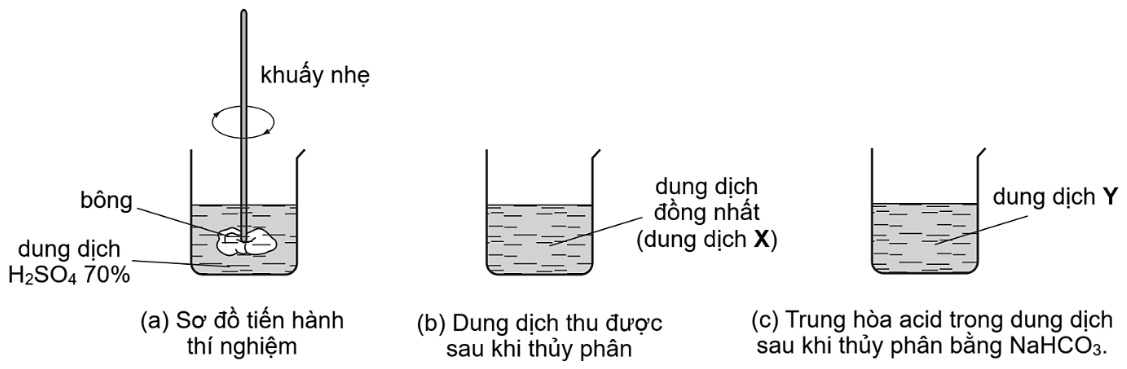
\includegraphics[height=3.4cm]{images_de_goc_11/image10_crop.png}
\end{center}
\vspace{2pt}
Dung dịch Y có chứa hỗn hợp các monosaccharide, disaccharide, trisaccharide,\dots{} do phản ứng thủy phân chưa hoàn toàn.
\vspace{3pt}

\begin{tabularx}{\linewidth}{@{}X r@{}}
a) Để tăng tốc độ và hiệu suất phản ứng thủy phân cellulose, thay dung dịch $\ce{H2SO4}\ 70\%$ bằng dung dịch $\ce{H2SO4}\ 98\%$. & $[\quad]$\\[4pt]
b) Disaccharide trong dung dịch Y là maltose và saccharose. & $[\quad]$\\[4pt]
c) Dung dịch X chứa monosaccharide duy nhất là glucose. & $[\quad]$\\[4pt]
d) Dung dịch Y làm mất màu dung dịch nước bromine. & $[\quad]$
\end{tabularx}
\vspace*{\fill}
\newpage

% SLIDE 16: CÂU 4 (Biodiesel từ dầu ăn thải)
\fontsize{23}{29}\selectfont
\textbf{Câu 4.} Biodiesel ($D = 0{,}88\text{ g/mL}$) là nhiên liệu lỏng thân thiện với môi trường, được sản xuất thông qua phản ứng giữa chất béo với alcohol mạch ngắn (xúc tác kiềm), thu được biodiesel (ester của acid béo) và glycerol ($D = 1{,}26\text{ g/mL}$). Một nhà máy tái chế dầu ăn thải để sản xuất biodiesel theo sơ đồ sau:
\begin{center}
$\ce{(RCOO)3C3H5 + 3CH3OH ->[xt] 3RCOOCH3 + C3H5(OH)3} \quad (1)$
\end{center}
\vspace{3pt}

\begin{tabularx}{\linewidth}{@{}X r@{}}
a) Biodiesel có thành phần nguyên tố giống dầu diesel truyền thống. & $[\quad]$\\[5pt]
b) Từ $500\text{ kg}$ một loại dầu ăn đã qua sử dụng có chứa $86\%$ chất béo (phân tử khối trung bình là $860\text{ amu}$), còn lại là tạp chất không chuyển hóa, có thể tạo tối đa $432\text{ kg}$ biodiesel dạng methyl ester với hiệu suất chuyển hóa $90\%$. & $[\quad]$\\[5pt]
c) Sau khi phản ứng (1) kết thúc, hỗn hợp sản phẩm phân thành hai lớp chất lỏng không đồng nhất, trong đó lớp biodiesel nổi lên trên bề mặt. & $[\quad]$\\[5pt]
d) Phương pháp trên giúp tận dụng dầu ăn đã qua sử dụng, giảm ô nhiễm môi trường do dầu ăn thải gây ra. & $[\quad]$
\end{tabularx}
\vspace*{\fill}
\newpage

% ==============================================================================
% PHẦN III. CÂU TRẮC NGHIỆM TRẢ LỜI NGẮN (1 CÂU / SLIDE)
% ==============================================================================

% SLIDE 17: CÂU 1
\fontsize{26}{34}\selectfont
\textbf{Câu 1.} Một học sinh gọi tên các ester như sau:
\vspace{6pt}

\begin{tabularx}{\linewidth}{@{}X X@{}}
(1) $\ce{HCOOCH3}$: methyl methanoate. & (2) $\ce{CH3CH2COOCH=CH2}$: vinyl propanoate.\\[6pt]
(3) $\ce{CH2=C(CH3)COOCH2CH3}$: ethyl methacrylate. & (4) $\ce{CH2=CHCOOCH2CH2CH3}$: isopropyl acrylate.\\[6pt]
(5) $\ce{CH3COOCH2CH2CH(CH3)2}$: isoamyl acetate. & (6) $\ce{C6H5COOCH2C6H5}$: phenyl benzoate.
\end{tabularx}
\vspace{10pt}
Số ester có tên gọi không đúng là bao nhiêu?
\vspace{20pt}

{\fontsize{30}{38}\selectfont \textbf{Trả lời:} $\dots\dots\dots\dots\dots\dots\dots\dots\dots\dots\dots\dots\dots\dots$}
\vspace*{\fill}
\newpage

% SLIDE 18: CÂU 2
\fontsize{25}{32}\selectfont
\textbf{Câu 2.} Hợp chất hữu cơ E mạch hở có công thức phân tử $\ce{C5H10O4}$. Cho sơ đồ phản ứng sau:
\vspace{4pt}

\begin{center}
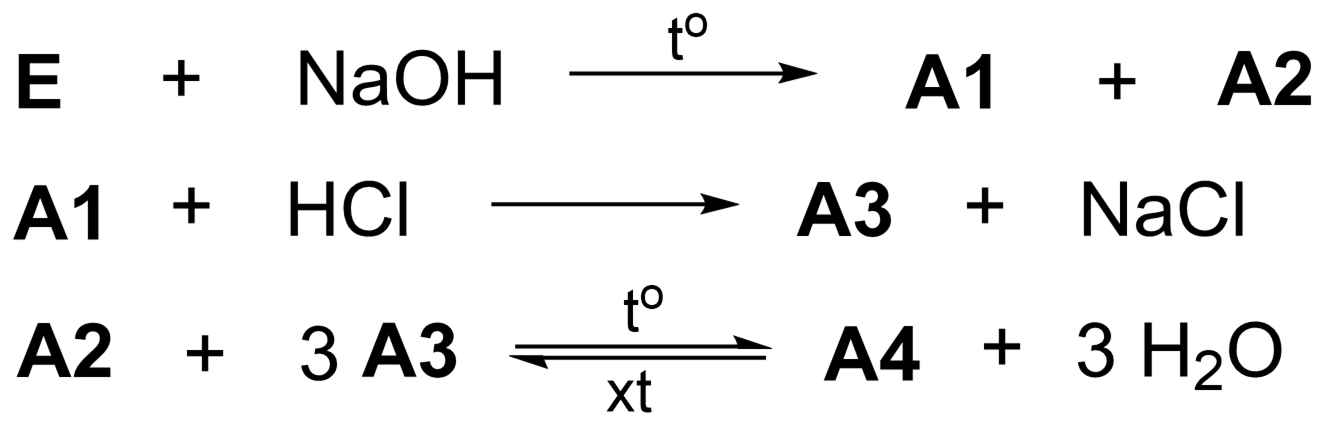
\includegraphics[height=2.8cm]{images_de_goc_11/cau2_p3_scheme_clean.png}
\end{center}
\vspace{2pt}
Dung dịch mỗi chất tan E, $\ce{A2}$ và $\ce{A3}$ đều có khả năng hòa tan $\ce{Cu(OH)2}$. Hợp chất $\ce{A4}$ có CTPT là $\ce{C9H14O6}$. Cho các nhận xét: (1) E chứa nhóm ketone; (2) Ở đkt, $\ce{A1}$ ở trạng thái rắn; (3) Phân tử khối $\ce{A3}$ là 74; (4) $\ce{A2}$ cho kết tủa vàng với $\ce{I2/NaOH}$; (5) $\ce{A4}$ là hợp chất đa chức. Liệt kê các nhận xét đúng theo thứ tự từ nhỏ đến lớn (viết liền).
\vspace{14pt}

{\fontsize{30}{38}\selectfont \textbf{Trả lời:} $\dots\dots\dots\dots\dots\dots\dots\dots\dots\dots\dots\dots\dots\dots$}
\vspace*{\fill}
\newpage

% SLIDE 19: CÂU 3
\fontsize{28}{38}\selectfont
\textbf{Câu 3.} Cho các amine có công thức cấu tạo dưới đây:
\vspace{6pt}

\begin{center}
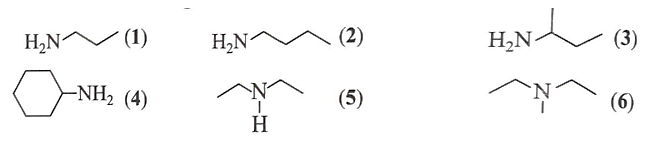
\includegraphics[height=3.4cm]{images_de_goc_11/image12_crop.png}
\end{center}
\vspace{10pt}
Có bao nhiêu amine bậc một trong dãy các amine trên?
\vspace{20pt}

{\fontsize{30}{38}\selectfont \textbf{Trả lời:} $\dots\dots\dots\dots\dots\dots\dots\dots\dots\dots\dots\dots\dots\dots$}
\vspace*{\fill}
\newpage

% SLIDE 20: CÂU 4
\fontsize{28}{38}\selectfont
\textbf{Câu 4.} Cho các chất sau:\\
\begin{center}
cellulose (1), saccharose (2), aniline (3), albumin (4), tristearin (5) và Gly-Ala-Val (6).
\end{center}
\vspace{10pt}
Có bao nhiêu chất bị thủy phân trong môi trường acid ở điều kiện thích hợp?
\vspace{22pt}

{\fontsize{30}{38}\selectfont \textbf{Trả lời:} $\dots\dots\dots\dots\dots\dots\dots\dots\dots\dots\dots\dots\dots\dots$}
\vspace*{\fill}
\newpage

% SLIDE 21: CÂU 5 (Đã chỉnh tránh overfull hbox)
\fontsize{24}{32}\selectfont
\textbf{Câu 5.} Monosodium glutamate (MSG) ($\ce{HOOC-CH2-CH2-CH(NH2)-COONa}$) là chất điều vị phổ biến (bột ngọt). Để tách MSG từ hỗn hợp thực phẩm, người ta kết tinh lại từ dung dịch nước bằng cách hạ nhiệt độ.\\[4pt]
Biết độ tan trong nước của MSG ở $60^\circ\text{C}$ là $112\text{ g}/100\text{ g}\ \ce{H2O}$; ở $25^\circ\text{C}$ là $74\text{ g}/100\text{ g}\ \ce{H2O}$. Tính khối lượng tinh thể (tấn) $\ce{HOOC-CH2-CH2-CH(NH2)-COONa.H2O}$ kết tinh khi làm nguội 2 tấn dung dịch bão hòa MSG ở $60^\circ\text{C}$ xuống $25^\circ\text{C}$ (kết quả làm tròn đến hàng phần trăm).
\vspace{20pt}

{\fontsize{30}{38}\selectfont \textbf{Trả lời:} $\dots\dots\dots\dots\dots\dots\dots\dots\dots\dots\dots\dots\dots\dots$}
\vspace*{\fill}
\newpage

% SLIDE 22: CÂU 6
\fontsize{25}{33}\selectfont
\textbf{Câu 6.} Cho phương trình hóa học của các phản ứng được đánh số thứ tự từ 1 tới 4:\\
\vspace{4pt}
\begin{tabularx}{\linewidth}{@{}l X@{}}
(1) & $\ce{CH3CHO + 2[Ag(NH3)2]OH -> CH3COONH4 + 2Ag v + 3NH3 + H2O}$\\[4pt]
(2) & $\ce{CH3CHO + 3I2 + 4NaOH -> CHI3 v + HCOONa + 3NaI + 3H2O}$\\[4pt]
(3) & $\ce{C6H12O6 ->[\text{men}] 2C2H5OH + 2CO2 ^}$\\[4pt]
(4) & $\ce{(C6H10O5)_n + nH2O ->[\text{enzyme}] nC6H12O6}$
\end{tabularx}
\vspace{6pt}
Gán số thứ tự PTHH của các phản ứng theo tên gọi: \textbf{Phản ứng với thuốc thử Tollens}, \textbf{phản ứng lên men rượu}, \textbf{phản ứng tạo iodoform}, \textbf{phản ứng thủy phân} và sắp xếp theo trình tự thành dãy bốn số (ví dụ: 1234, 4321,\dots).
\vspace{18pt}

{\fontsize{30}{38}\selectfont \textbf{Trả lời:} $\dots\dots\dots\dots\dots\dots\dots\dots\dots\dots\dots\dots\dots\dots$}
\vspace*{\fill}
\newpage

% ==============================================================================
% SLIDE 23: BẢNG ĐÁP ÁN TỔNG HỢP (Gọn gàng vừa khít 1 slide)
% ==============================================================================
\begin{center}
{\fontsize{22}{26}\selectfont \textbf{\color{brandGreen}BẢNG ĐÁP ÁN -- ĐỀ KIỂM TRA ĐỊNH KÌ HÓA 12 (ĐỀ GỐC LẦN 11)}}\\[0.15cm]
\end{center}

\fontsize{15}{18}\selectfont
\textbf{PHẦN I. Trắc nghiệm nhiều phương án lựa chọn (18 câu):}\\[2pt]
\renewcommand{\arraystretch}{1.1}
\begin{tabularx}{\linewidth}{|c|*{9}{>{\centering\arraybackslash}X|}}
\hline
\textbf{Câu} & \textbf{1} & \textbf{2} & \textbf{3} & \textbf{4} & \textbf{5} & \textbf{6} & \textbf{7} & \textbf{8} & \textbf{9} \\
\hline
\textbf{Đ/A} & \textbf{\color{brandRed}C} & \textbf{\color{brandRed}B} & \textbf{\color{brandRed}D} & \textbf{\color{brandRed}D} & \textbf{\color{brandRed}D} & \textbf{\color{brandRed}B} & \textbf{\color{brandRed}A} & \textbf{\color{brandRed}A} & \textbf{\color{brandRed}B} \\
\hline
\textbf{Câu} & \textbf{10} & \textbf{11} & \textbf{12} & \textbf{13} & \textbf{14} & \textbf{15} & \textbf{16} & \textbf{17} & \textbf{18} \\
\hline
\textbf{Đ/A} & \textbf{\color{brandRed}C} & \textbf{\color{brandRed}A} & \textbf{\color{brandRed}D} & \textbf{\color{brandRed}C} & \textbf{\color{brandRed}C} & \textbf{\color{brandRed}C} & \textbf{\color{brandRed}A} & \textbf{\color{brandRed}C} & \textbf{\color{brandRed}C} \\
\hline
\end{tabularx}
\vspace{4pt}

\textbf{PHẦN II. Trắc nghiệm Đúng / Sai (4 câu):}\\[2pt]
\begin{tabularx}{\linewidth}{|c|*{4}{>{\centering\arraybackslash}X|}}
\hline
\textbf{Ý} & \textbf{Câu 1 (Ester hóa)} & \textbf{Câu 2 (Methionine)} & \textbf{Câu 3 (Thủy phân cellulose)} & \textbf{Câu 4 (Biodiesel)} \\
\hline
\textbf{a)} & \textbf{Sai} ($\ce{HCl}$ bay hơi) & \textbf{Sai} (có 11 H) & \textbf{Sai} ($\ce{H2SO4}$ đặc làm than hóa) & \textbf{Sai} (chứa C, H, O) \\
\hline
\textbf{b)} & \textbf{\color{brandRed}Đúng} ($H = 50\%$) & \textbf{\color{brandRed}Đúng} ($\alpha$-amino acid) & \textbf{Sai} (tạo cellobiose) & \textbf{Sai} (tính ra $388{,}8\text{ kg}$) \\
\hline
\textbf{c)} & \textbf{\color{brandRed}Đúng} ($t_{\text{s}} = 34{,}6^\circ\text{C}$) & \textbf{\color{brandRed}Đúng} (thịt, cá, trứng) & \textbf{\color{brandRed}Đúng} (monosaccharide duy nhất) & \textbf{\color{brandRed}Đúng} (nổi lên trên) \\
\hline
\textbf{d)} & \textbf{Sai} (phản ứng ester hóa) & \textbf{\color{brandRed}Đúng} (IUPAC chuẩn) & \textbf{\color{brandRed}Đúng} (làm mất màu $\ce{Br2}$) & \textbf{\color{brandRed}Đúng} (bảo vệ môi trường) \\
\hline
\end{tabularx}
\vspace{4pt}

\textbf{PHẦN III. Trắc nghiệm trả lời ngắn (6 câu):}\\[2pt]
\begin{tabularx}{\linewidth}{|c|*{6}{>{\centering\arraybackslash}X|}}
\hline
\textbf{Câu} & \textbf{Câu 1} & \textbf{Câu 2} & \textbf{Câu 3} & \textbf{Câu 4} & \textbf{Câu 5} & \textbf{Câu 6} \\
\hline
\textbf{Đáp số} & \textbf{\color{brandRed}2} & \textbf{\color{brandRed}25} & \textbf{\color{brandRed}4} & \textbf{\color{brandRed}5} & \textbf{\color{brandRed}0,43} & \textbf{\color{brandRed}1324} \\
\hline
\end{tabularx}

\end{document}
